\documentclass[12pt]{article}
%%%%%%%%%%%%%%%%%%%%%%%%%%%%%%%%%%%%%%%%%
% Cleese Assignment
% Structure Specification File
% Version 1.0 (27/5/2018)
%
% This template originates from:
% http://www.LaTeXTemplates.com
%
% Author:
% Vel (vel@LaTeXTemplates.com)
%
% License:
% CC BY-NC-SA 3.0 (http://creativecommons.org/licenses/by-nc-sa/3.0/)
% 
%%%%%%%%%%%%%%%%%%%%%%%%%%%%%%%%%%%%%%%%%

%----------------------------------------------------------------------------------------
%	PACKAGES AND OTHER DOCUMENT CONFIGURATIONS
%----------------------------------------------------------------------------------------

\usepackage{lastpage} % Required to determine the last page number for the footer

\usepackage{graphicx} % Required to insert images

\setlength\parindent{0pt} % Removes all indentation from paragraphs

\usepackage[most]{tcolorbox} % Required for boxes that split across pages

\usepackage{booktabs} % Required for better horizontal rules in tables

\usepackage{listings} % Required for insertion of code

\usepackage{etoolbox} % Required for if statements

%----------------------------------------------------------------------------------------
%	MARGINS
%----------------------------------------------------------------------------------------

\usepackage{geometry} % Required for adjusting page dimensions and margins

\geometry{
	paper=a4paper, % Change to letterpaper for US letter
	top=3cm, % Top margin
	bottom=3cm, % Bottom margin
	left=2.5cm, % Left margin
	right=2.5cm, % Right margin
	headheight=14pt, % Header height
	footskip=1.4cm, % Space from the bottom margin to the baseline of the footer
	headsep=1.2cm, % Space from the top margin to the baseline of the header
	%showframe, % Uncomment to show how the type block is set on the page
}

%----------------------------------------------------------------------------------------
%	FONT
%----------------------------------------------------------------------------------------

\usepackage[utf8]{inputenc} % Required for inputting international characters
\usepackage[T1]{fontenc} % Output font encoding for international characters

\usepackage[sfdefault,light]{roboto} % Use the Roboto font

%----------------------------------------------------------------------------------------
%	HEADERS AND FOOTERS
%----------------------------------------------------------------------------------------

\usepackage{fancyhdr} % Required for customising headers and footers

\pagestyle{fancy} % Enable custom headers and footers

\lhead{\small\assignmentClass\ifdef{\assignmentClassInstructor}{\ (\assignmentClassInstructor):}{}\ \assignmentTitle} % Left header; output the instructor in brackets if one was set
\chead{} % Centre header
\rhead{\small\ifdef{\assignmentAuthorName}{\assignmentAuthorName}{\ifdef{\assignmentDueDate}{Due\ \assignmentDueDate}{}}} % Right header; output the author name if one was set, otherwise the due date if that was set

\lfoot{} % Left footer
\cfoot{\small Page\ \thepage\ of\ \pageref{LastPage}} % Centre footer
\rfoot{} % Right footer

\renewcommand\headrulewidth{0.5pt} % Thickness of the header rule

%----------------------------------------------------------------------------------------
%	MODIFY SECTION STYLES
%----------------------------------------------------------------------------------------

\usepackage{titlesec} % Required for modifying sections

%------------------------------------------------
% Section

\titleformat
{\section} % Section type being modified
[block] % Shape type, can be: hang, block, display, runin, leftmargin, rightmargin, drop, wrap, frame
{\Large\bfseries} % Format of the whole section
{\assignmentQuestionName~\thesection} % Format of the section label
{6pt} % Space between the title and label
{} % Code before the label

\titlespacing{\section}{0pt}{0.5\baselineskip}{0.5\baselineskip} % Spacing around section titles, the order is: left, before and after

%------------------------------------------------
% Subsection

\titleformat
{\subsection} % Section type being modified
[block] % Shape type, can be: hang, block, display, runin, leftmargin, rightmargin, drop, wrap, frame
{\itshape} % Format of the whole section
{(\alph{subsection})} % Format of the section label
{4pt} % Space between the title and label
{} % Code before the label

\titlespacing{\subsection}{0pt}{0.5\baselineskip}{0.5\baselineskip} % Spacing around section titles, the order is: left, before and after

\renewcommand\thesubsection{(\alph{subsection})}

%----------------------------------------------------------------------------------------
%	CUSTOM QUESTION COMMANDS/ENVIRONMENTS
%----------------------------------------------------------------------------------------

% Environment to be used for each question in the assignment
\newenvironment{question}{
	\vspace{0.5\baselineskip} % Whitespace before the question
	\section{} % Blank section title (e.g. just Question 2)
	\lfoot{\small\itshape\assignmentQuestionName~\thesection~continued on next page\ldots} % Set the left footer to state the question continues on the next page, this is reset to nothing if it doesn't (below)
}{
	\lfoot{} % Reset the left footer to nothing if the current question does not continue on the next page
}

%------------------------------------------------

% Environment for subquestions, takes 1 argument - the name of the section
\newenvironment{subquestion}[1]{
	\subsection{#1}
}{
}

%------------------------------------------------

% Command to print a question sentence
\newcommand{\questiontext}[1]{
	\textbf{#1}
	\vspace{0.5\baselineskip} % Whitespace afterwards
}

%------------------------------------------------

% Command to print a box that breaks across pages with the question answer
\newcommand{\answer}[1]{
	\begin{tcolorbox}[breakable, enhanced]
		#1
	\end{tcolorbox}
}

%------------------------------------------------

% Command to print a box that breaks across pages with the space for a student to answer
\newcommand{\answerbox}[1]{
	\begin{tcolorbox}[breakable, enhanced]
		\vphantom{L}\vspace{\numexpr #1-1\relax\baselineskip} % \vphantom{L} to provide a typesetting strut with a height for the line, \numexpr to subtract user input by 1 to make it 0-based as this command is
	\end{tcolorbox}
}

%------------------------------------------------

% Command to print an assignment section title to split an assignment into major parts
\newcommand{\assignmentSection}[1]{
	{
		\centering % Centre the section title
		\vspace{2\baselineskip} % Whitespace before the entire section title
		
		\rule{0.8\textwidth}{0.5pt} % Horizontal rule
		
		\vspace{0.75\baselineskip} % Whitespace before the section title
		{\LARGE \MakeUppercase{#1}} % Section title, forced to be uppercase
		
		\rule{0.8\textwidth}{0.5pt} % Horizontal rule
		
		\vspace{\baselineskip} % Whitespace after the entire section title
	}
}

%----------------------------------------------------------------------------------------
%	TITLE PAGE
%----------------------------------------------------------------------------------------

\author{\textbf{\assignmentAuthorName}} % Set the default title page author field
\date{} % Don't use the default title page date field

\title{
	\thispagestyle{empty} % Suppress headers and footers
	\vspace{0.2\textheight} % Whitespace before the title
	\textbf{\assignmentClass:\ \assignmentTitle}\\[-4pt]
	\ifdef{\assignmentDueDate}{{\small Due\ on\ \assignmentDueDate}\\}{} % If a due date is supplied, output it
	\ifdef{\assignmentClassInstructor}{{\large \textit{\assignmentClassInstructor}}}{} % If an instructor is supplied, output it
	\vspace{0.32\textheight} % Whitespace before the author name
}
 % Include the file specifying the document structure and custom commands
\newcommand{\assignmentQuestionName}{Question} % The word to be used as a prefix to question numbers; example alternatives: Problem, Exercise
\newcommand{\assignmentClass}{18-785} % Course/class
\newcommand{\assignmentTitle}{Assignment\ \#5} % Assignment title or name
\newcommand{\assignmentAuthorName}{Junxiao Guo} % Student name

% Optional (comment lines to remove)
%\newcommand{\assignmentDueDate}{Monday,\ October\ 31,\ 2019} % Due date

\begin{document}
	
	% --------------------------------------------------------------
	%                         Start here
	% --------------------------------------------------------------
	
	\title{18-785 Data, Interference, and Applied Machine Learning \\ Homework Assignment 5}
	\author{Junxiao Guo \\ Andrew ID: junxiaog}
	
	\maketitle
	
	% --------------------------------------------------------------
	%     You don't have to mess with anything below this line.
	% --------------------------------------------------------------
	%----------------------------------------------------------------------------------------
	%	QUESTION 1
	%----------------------------------------------------------------------------------------
	

	\section{Statistical learning}
	\subsection{1.1 Rule-based approach}
	\questiontext{Four steps to implementing a rule-based approach}
	\answer{
	\begin{enumerate}
	\item A list of rules or rule base, which is a specific type of knowledge base.
	\item An inference engine or semantic reasoner, which infers information or takes action based on the interaction of input and the rule base. The interpreter executes a production system program by performing the following match-resolve-act cycle.
	\item Temporary working memory.
	\item A user interface or other connection to the outside world through which input and output signals are received and sent.
	\end{enumerate}
	}
	\questiontext{Domain knowledge required to establish a rule}
	\answer{
	}
	\subsection{1.2 Over-fitting}
	\questiontext{Explain over-fitting and why it is a problem in statistical learning}\\\\
	\answer{
	\underline{Over-fitting}: In statistics, over-fitting is "the production of an analysis that corresponds too closely or exactly to a particular set of data, and may therefore fail to fit additional data or predict future observations reliably". An over-fitted model is a statistical model that contains more parameters than can be justified by the data.The essence of over-fitting is to have unknowingly extracted some of the residual variation (i.e. the noise) as if that variation represented underlying model structure.}
	\answer{
	\underline{Why Problematic}: Over-fitted model can not obtain truly unbiased sample of population of any data. The over-fitted model is likely to be biased to the sample instead of predicting the parameters for the entire data population.}


	\questiontext{Dealing with small datasets}
	\answer{
	\underline{For small datasets}: If we only have a small datasets of ten data points, we \textbf{should use s simple model} because if we use a complex model, it will be easily get over-fitted because complex model can easily be trained to fit every data-points from the small datasets, which will lose the generality of our model.}
	\subsection{1.3 Commonly used approaches to avoid over-fitting}
	\answer{
	\textbf{Simplifying the model}: make sure that the number of independent parameters in your fit is much smaller than the number of data points you have.  By independent parameters, I mean the number of coefficients in a polynomial or the number of weights and biases in a neural network, not the number of independent variables
	\\\\
	\textbf{Adding Regularizations}: Regularization attempts to reduce the variance of the estimator by simplifying it, something that will increase the bias, in such a way that the expected error decreases
	}

	
	\subsection{1.4 Metrics used to evaluate the performance}
	\answer{
	\textbf{F1 Score}\\
	F1 is an overall measure of a model's accuracy that combines precision and recall, in that weird way that addition and multiplication just mix two ingredients to make a separate dish altogether.
	$${F_1}= {(recall^{-1}+precision^{-1})\over{2}}^{-1}=2\cdot{precision\cdot recall\over{precision+recall}}$$
	For the precision and recall for F1 Score: 
	$$Precision={TruePositive \over {TruePositive + FalsePostiive}}$$
	$$Recall = {TruePositive \over {TruePositive+FalseNegative}}$$
	\\
	\\
	\textbf{R-Squared}\\
	R-squared, also known as the coefficient of determination, is the statistical measurement of the correlation between an investment’s performance and a specific benchmark index. In other words, it shows what degree a stock or portfolio’s performance can be attributed to a benchmark index.
	$$R^2=1-{MSE(model)\over{MSE(baseline)}}$$
	
	MSE(model) = Mean Squared Error of the predictions against the actual values
	$$MSE(model)=\sum_i^N(y_i-\hat{y})^2$$
	
	MSE(baseline) = Mean Squared Error of  mean prediction against the actual values
	$$MSE(model)=\sum_i^N(\bar{y_i}-\hat{y})^2$$}
\answer{
	\textbf{Examples}\\
	\textbullet { Evaluation of named entity recognition and word segmentation: F1 Score}\\
	\textbullet { Representing how a funds movements correlates with a benchmark index: R-Squared}
	}
	
	\subsection{1.5 Why Benchmark}
	\answer{
	1. Benchmark is standard against which you compare the solutions, to get a feel if the solutions are better or worse.\\\\
	2. When the benchmarks are “representative,” they allow engineering effort to be focused on a small but high-value and widely used set of targets. In the best cases, benchmarks initiate a virtuous circle, propelling a cycle of optimization and improved value for all members of a community}
\answer{
	\textbf{Examples for benchmark}\\
	1. 
}
	

	
	\newpage
	\section{Machine Learning}
	\subsection{2.1 What is Machine Learning \& Why Machine Learning}
	\answer{
	\textbf{What is machine learning}\\
	Machine learning (ML) is the scientific study of algorithms and statistical models that computer systems use to perform a specific task without using explicit instructions, relying on patterns and inference instead. It is seen as a subset of artificial intelligence. Machine learning algorithms build a mathematical model based on sample data, known as "training data", in order to make predictions or decisions without being explicitly programmed to perform the task. Machine learning algorithms are used in a wide variety of applications, such as email filtering and computer vision, where it is difficult or infeasible to develop a conventional algorithm for effectively performing the task.}
	\answer{
	\textbf{Evolution over time}\\
	\textbullet Alan Turing Test(1950) :  A machine can actually learn, if when we communicate with it, we cannot distinguish it from another human.\\
	\textbullet ELIZA(1952) : Arthur Samuel (IBM) wrote the first game-playing program, ELIZA, for checkers, to achieve sufficient skill to challenge a world champion.\\
	\textbullet Neural Network(1957): Frank Rosenblatt (Cornell University) invented the perceptron, a very simple linear classifier.\\
	\textbullet Artificial Intelligence(1990): Computer science and statistics combined to provide a data-driven approach to machine learning.\\
	\textbullet 	Big Data(2010): Exponential growth in the volume, velocity and variety of data available for analysis and research.\\
	\textbullet Open Data(2014): Infrastructure, protocols and standards for providing open access to data.
	}
	

	\subsection{2.2 Examples of machine learning techniques}
	\answer{
	\textbullet Decision Tree (Supervised)\\
	\textbullet Linear Regression (Supervised)\\
	\textbullet K-means (Unsupervised)\\
}
	\subsection{2.3 Classification \& Regression}
	\answer{
	The main difference between them is that the output variable in regression is numerical (or continuous) while that for classification is categorical (or discrete)}
	
	\subsection{2.4 Supervised \& Unsupervised learning}
	\answer{
	\textbf{Supervised}: All data is labeled and the algorithms learn to predict the output from the input data. \\
	\textbf{Unsupervised}: All data is unlabeled and the algorithms learn to inherent structure from the input data.
}
	
	\subsection{2.5 Examples}
	\questiontext{Examples of successful applications of machine learning and technique involved}
	\answer{
	\textbullet \textbf{Facial Recognition}: Convoluted Neural Network\\
	\textbullet \textbf{Speech Recognition}: Recurrent Neural Network\\
}	
	
	
	\section{Diabetes data}
	\subsection{3.1 Correlation \& Heat-Map}
	\answer{
	\textbf{Correlation Matrix}
	\begin{center}
		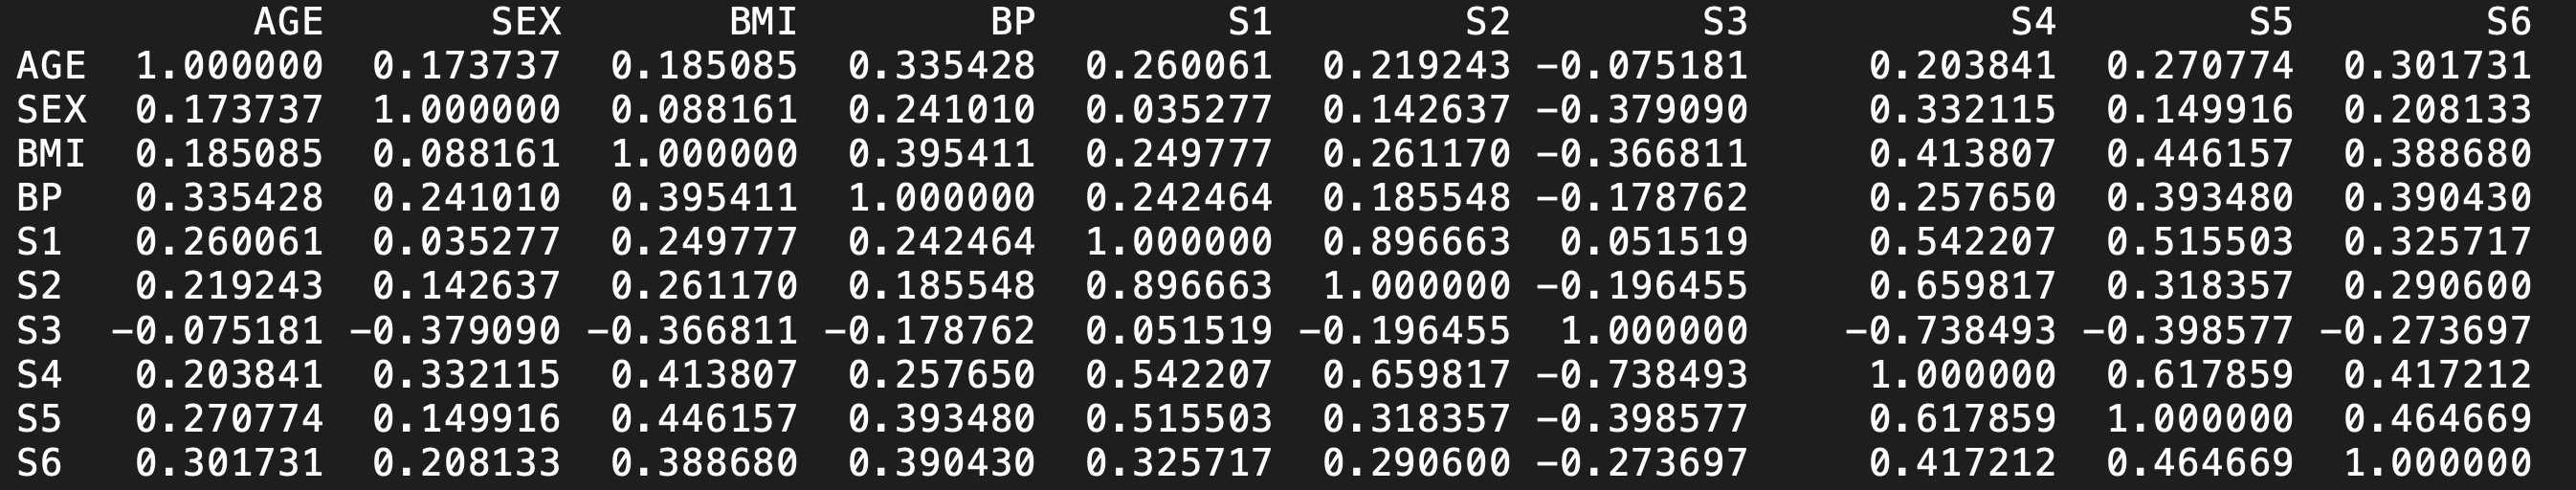
\includegraphics[width=0.9\columnwidth]{hw5_p3q2.png}
	\end{center}
	\textbf{Heat-map of the Matrix}
	\begin{center}
	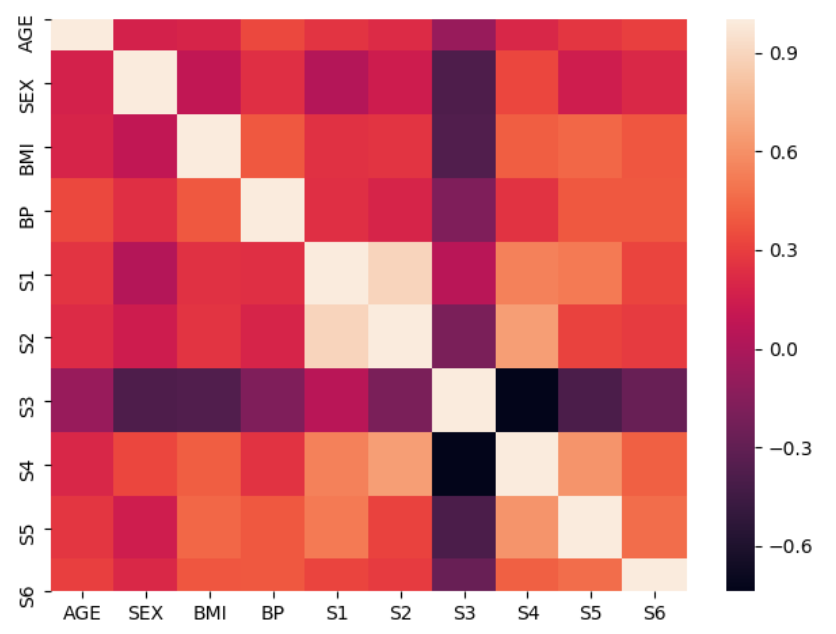
\includegraphics[width=0.5\columnwidth]{hw5_p3q1.png}
	\end{center}
	}

	\subsection{3.2 Collinearity}
	\answer{
		\underline{What is collinearity}\\
		Collinearity, in statistics, correlation between predictor variables (or independent variables), such that they express a linear relationship in a regression model.
		\underline{Effects of collinearity}\\
		When predictor variables in the same regression model are correlated, they cannot independently predict the value of the dependent variable. In other words, they explain some of the same variance in the dependent variable, which in turn reduces their statistical significance.
	}

	\subsection{3.3 Multivariate Model}
	\answer{
	\textbf{Model1 Result}
	\begin{center}
		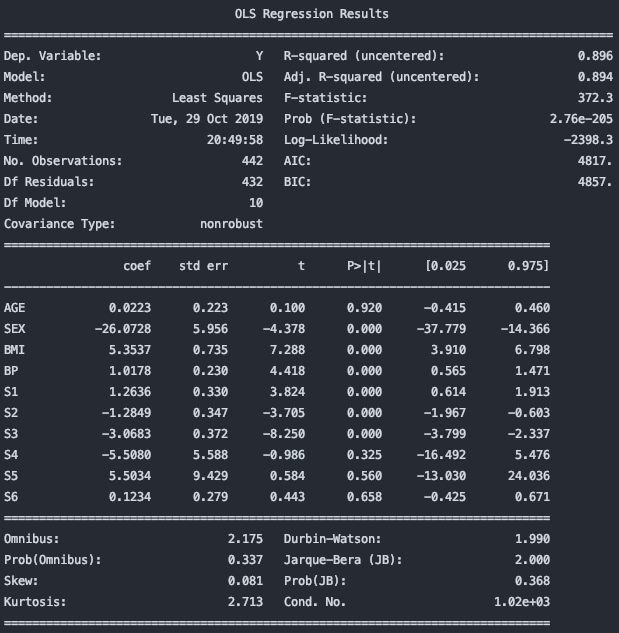
\includegraphics[width=0.8\columnwidth]{hw5_p3q3.png}
	\end{center}
	\textbf{Mean Square Error \& Adjusted $R^2$}
	$$Mean Square Error = 3022.9210178861667$$
	$$Adjusted R^2 = 0.894$$
	
	\textbf{Are all variables significant? Could this be a problem of collinearity?}

	Based on the model1 result, there are only couple features are significant:
	\begin{itemize}
		\item 'Age', 'S4', 'S5', 'S6'	
	\end{itemize}
	And this should not cause problem of collinearity since the correlation between those features do not have dramatic difference.
	
	}
	
	\subsection{3.4 Difference between forward \& backward selection}
	\answer{
	\underline{Forward Selection}\\
	Start with a null model and add predictors to the model.\\
	\underline{Backward Selection}\\
	Start with a full model including all variables and then drop those are not significant, and drops one at a time.
	}
	\subsection{3.5 Stepwise Approach}
	\answer{
		By using stepwise method, the selected variables are:
		\begin{itemize}
			\item 'BMI', 'S5', 'BP', 'S1', 'SEX', 'S2'
		\end{itemize}
		\underline{Summary of StepWise Model}
		\begin{center}
			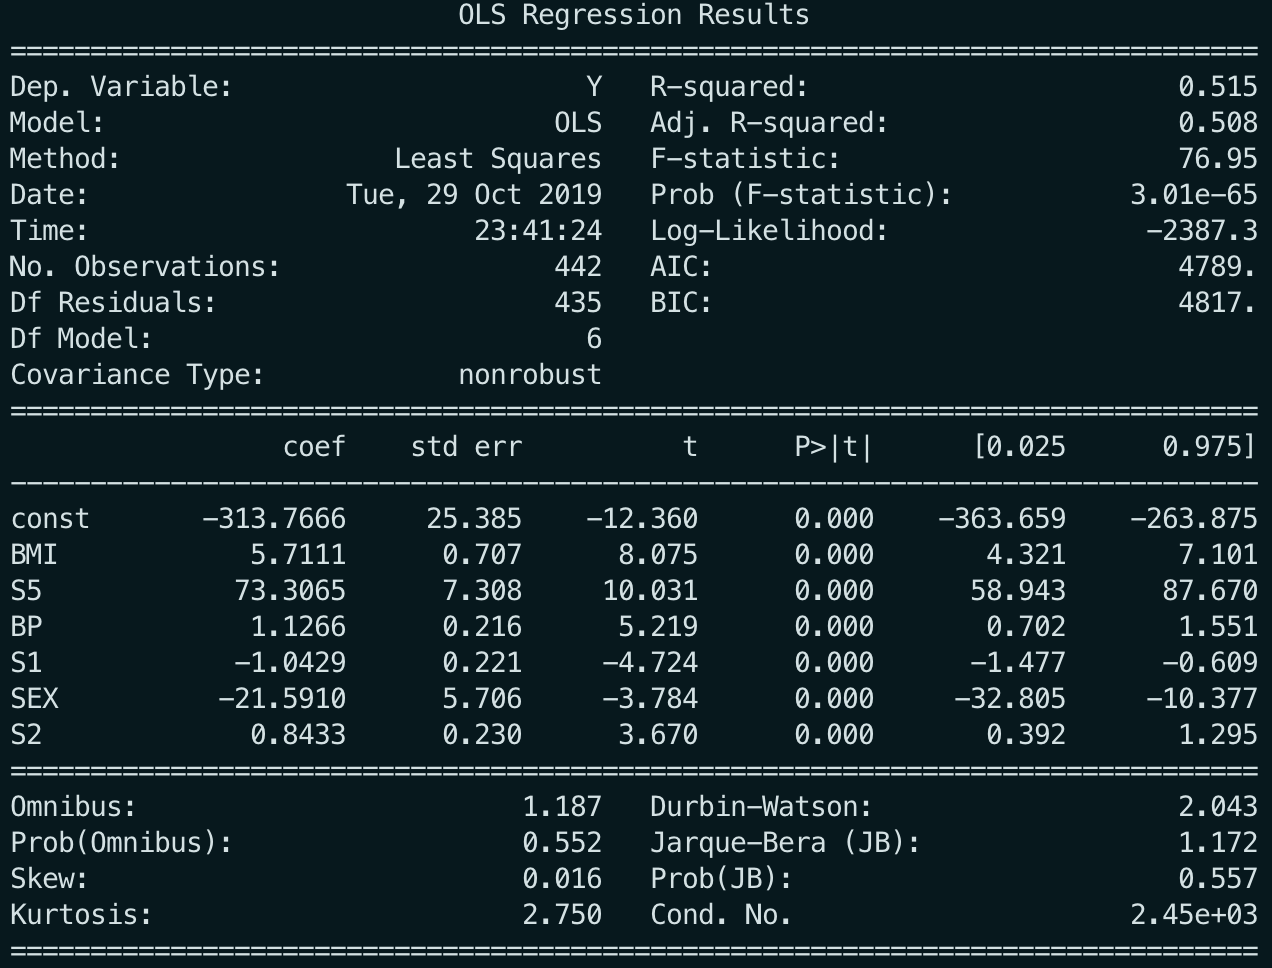
\includegraphics[width=0.8\columnwidth]{hw5_p3q5.png}
		\end{center}
		$$MeanSqureError = 2876.683251787016$$
		$$AdjustedR^2 = 0.508$$
	}
	
	
	\section{Analyzing the Titanic data set}
	\subsection{4.1 Logistic Regression \& Linear Regression}
	\answer{
	\underline{Linear Regression}
	\begin{itemize}
		\item Uses the linear equation $Y=b_0+\sum{(b_iX_i)}+\epsilon$ where $Y$ is a continuous dependent variable and independent variables $X_i$ are usually continuous (but can also be binary) or other discrete domains.
  		\item will be used when the dependent variable is binary in nature
	\end{itemize}
	\underline{Logistic Regression}
	\begin{itemize}
		\item start with a full model including all variables and then drop those you do not need/ are not significant 1 at a time.
		\item It is a generalized linear model procedure using the same basic formula, but instead of the continuous $Y$, it is regressing for the probability of a categorical outcome.
	\end{itemize}}
	\subsection{4.2 Probability of Survival}
	\answer{Titanic survival probability is :0.3819709702062643}
	\subsection{4.3 Table of Survival Probability}
	\answer{
	\begin{itemize}
		\item Children(0-14 Years):0.5700934579439252
		\item Youth(15-24 Years):0.3879598662207358
		\item Adults(25-64 Years):0.3974358974358974
		\item Senior(65 Years and older):0.15384615384615385
	\end{itemize}
	
	}
	\subsection{4.4 Logistic Regression Model for Survival Rates}
	\answer{	
	\underline {Model Result}\\
	\textbf{Note}:	2 and 3 represent passenger class, since we only need $n-1$ labels for each feature, so we only picked if the person is a male and if the person has passenger class of 2 or 3, and they can fully represent all the conditions.
	\begin{center}

		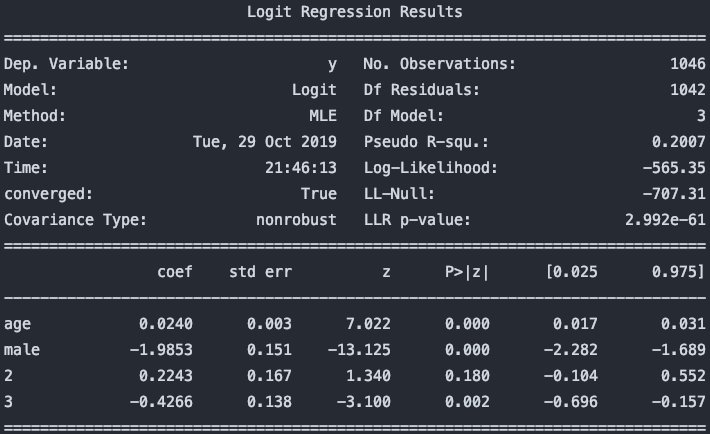
\includegraphics[width=0.8\columnwidth]{hw5_p4q4.png}
	\end{center}
	\underline{Parameter estimates \& parameters significancy}\\
	\textbf{Note}: Determine the significancy is based on the P value and Z value
	\begin{itemize}
		\item Age (Not Significant)
		\item If the person is male (Not Siginificant)
		\item If the person's passenger class is 2 (Significant)
		\item If the person's passenger class is 3 (Significant)
	\end{itemize}
	}
	\subsection{4.5 Model Performance}
	\answer{
	\underline{Classification Accuracy Based on Confusion Matrix}
		\begin{center}

		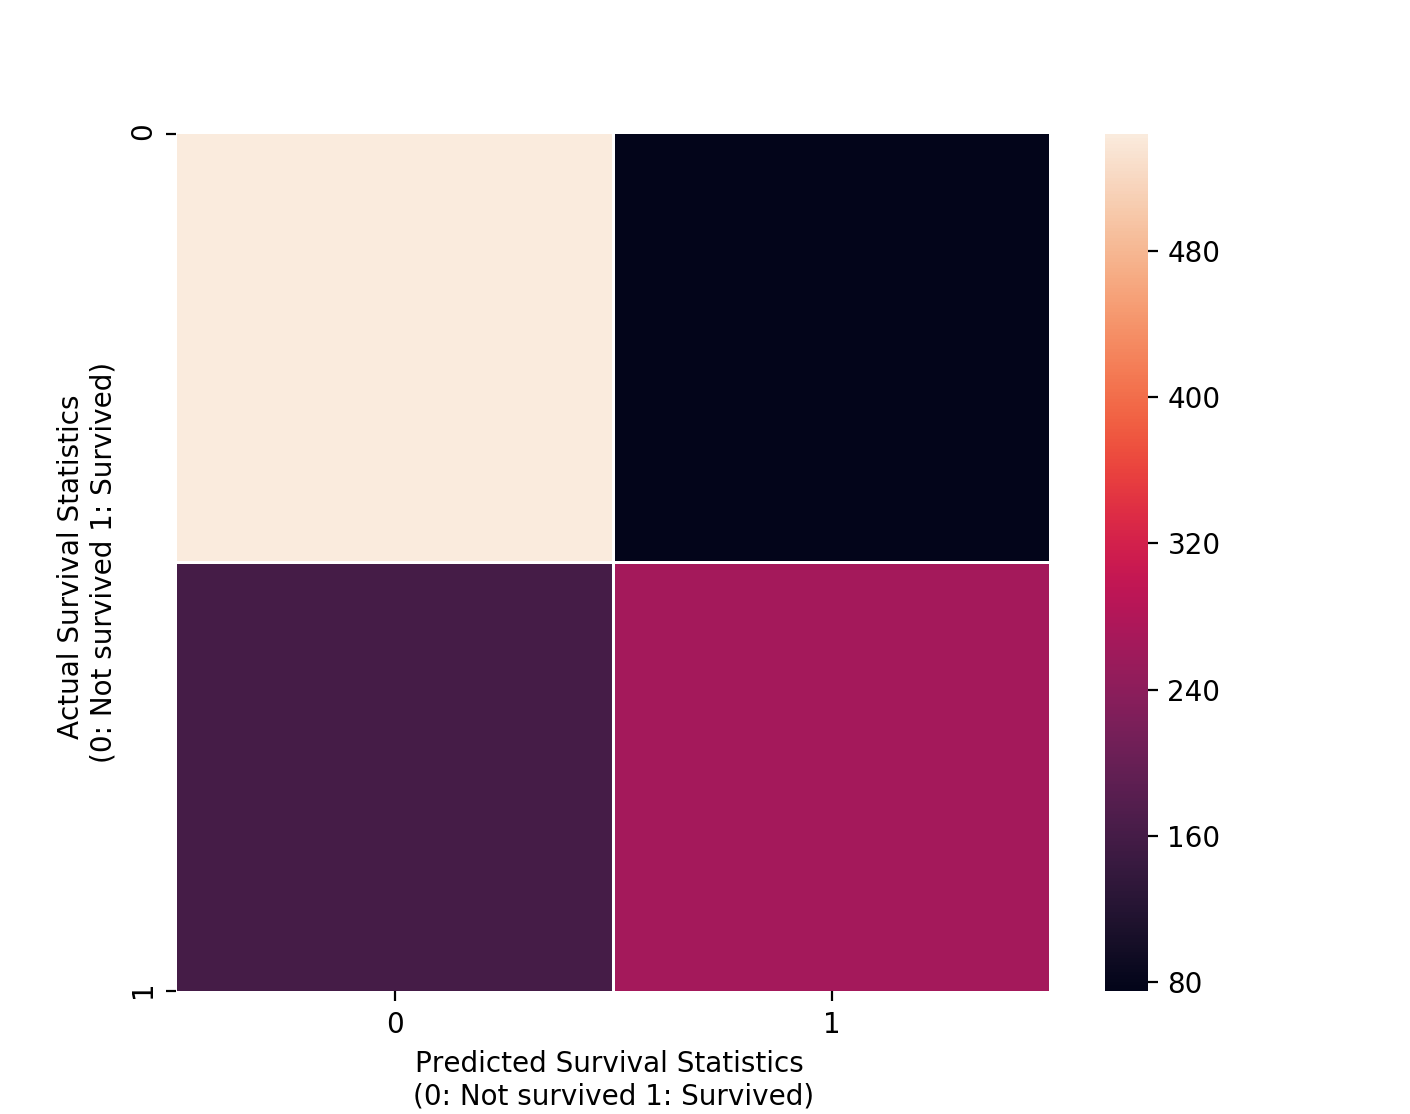
\includegraphics[width=0.8\columnwidth]{hw5_p4q5.png}
	\end{center}
	}
	
\end{document}